\documentclass{amsart}
\input{decls}
\usetikzlibrary {arrows.meta,backgrounds,fit,positioning}
\title{Graphs}
\author{Frank Tsai}
\date{\today}
%\thanks{}
\begin{document}
\maketitle
\tableofcontents

\section{Graphs}
\label{sec:graphs}

\begin{defn}
  \label{defn:graphs}
  A (directed) \emph{graph} $G$ consists of the following data:
  \begin{enumerate}
  \item A set $V$ of \emph{vertices}.
  \item A set $E \subseteq V \times V$ of \emph{edges}.
  \end{enumerate}
\end{defn}

\begin{rmk}
  \label{rmk:edges-are-binary-relations}
  Recall that a binary relation on a set $V$ can be encoded as any subset of $V \times V$.
  Thus, a graph is a set $V$ equipped with a binary relation $E$.
\end{rmk}

\begin{eg}
  \label{eg:graphs-example1}
  Let $V = \{A, B, C\}$ and $E = \{(A,B),(B,A),(B,C),(C,A)\}$.
  \begin{center}
    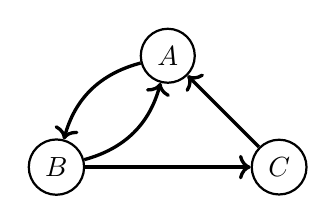
\begin{tikzpicture}[node distance= 2cm]
      \begin{scope}[every node/.style={circle,thick,draw}]
        \node (A) {$A$};
        \node (B) [below left of= A] {$B$};
        \node (C) [below right of=A] {$C$};
      \end{scope}
      \begin{scope}[every edge/.style={draw= black, very thick}]
        \path[->] (A) edge[bend right= 30] (B);
        \path[->] (B) edge[bend right= 30] (A);
        \path[->] (B) edge (C);
        \path[->] (C) edge (A);
      \end{scope}
    \end{tikzpicture}
  \end{center}
\end{eg}

\begin{defn}
  \label{defn:graphs-undirected}
  A graph $(V,E)$ is \emph{undirected} if the binary relation $E$ is symmetric.
\end{defn}

\begin{rmk}
  \label{rmk:example1-not-undirected}
  \cref{eg:graphs-example1} is not an undirected graph since $(B,C) \in E$, but $(C,B) \notin E$.
  Similarly, $(C,A) \in E$, but $(A,C) \notin E$.
\end{rmk}

\begin{rmk}
  \label{rmk:drop-arrows-in-undirected-graphs}
  In an undirected graph, we drop the arrow tips as they convey no additional information.
\end{rmk}

\begin{eg}
  \label{eg:graphs-example2}
  Let $V = \{A, B, C\}$ and $E = V \times V$.
  Note that $E$ is symmetric.
  \begin{center}
    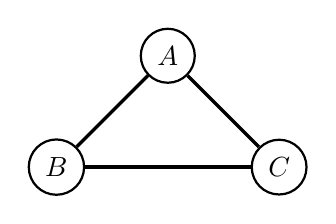
\begin{tikzpicture}[node distance= 2cm]
      \begin{scope}[every node/.style={circle,thick,draw}]
        \node (A) {$A$};
        \node (B) [below left of= A] {$B$};
        \node (C) [below right of=A] {$C$};
      \end{scope}
      \begin{scope}[every edge/.style={draw= black, very thick}]
        \path (A) edge (B);
        \path (A) edge (C);
        \path (B) edge (C);
      \end{scope}
    \end{tikzpicture}
  \end{center}
\end{eg}

\begin{defn}
  \label{defn:walks}
  Let $G = (V,E)$ be a graph.
  A \emph{walk} is a sequence of vertices and edges defined inductively as follows:
  \begin{enumerate}
  \item The empty sequence is a walk.
  \item If $(v_{1},v_{2}) \in E$ then the sequence $v_{1},(v_{1},v_{2}),v_{2}$ is a walk.
  \item If $(v_{n}, v_{m}) \in E$ and $v_{1},(v_{1},v_{2}),v_{2},\ldots,v_{n}$ is a walk then the sequence
    \[
      v_{1},(v_{1},v_{2}),v_{2},\ldots,v_{n},(v_{n},v_{m}),v_{m}
    \]
    is a walk.
  \end{enumerate}
\end{defn}

\begin{defn}
  \label{defn:walks-length}
  The \emph{length} of a walk is the number of edges in that walk.
\end{defn}

\begin{eg}
  \label{eg:walk-example-1}
  Let $G$ be the graph defined in \cref{eg:graphs-example2}.
  The sequence
  \[
    A,(A,B),B,(B,C),C,(C,A),A,(A,B),B
  \]
  is a walk.
  \begin{center}
    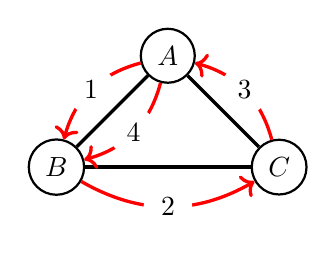
\begin{tikzpicture}[node distance= 2cm]
      \begin{scope}[every node/.style={circle,thick,draw}]
        \node (A) {$A$};
        \node (B) [below left of= A] {$B$};
        \node (C) [below right of=A] {$C$};
      \end{scope}
      \begin{scope}
        [every edge/.style={draw= black, very thick},
        every node/.style={fill=white,circle}]
        \path (A) edge (B);
        \path (A) edge (C);
        \path (B) edge (C);
        \path[->] (A) edge[draw= red, bend right= 30] node {$1$} (B);
        \path[->] (B) edge[draw= red, bend right= 30] node {$2$} (C);
        \path[->] (C) edge[draw= red, bend right= 30] node {$3$} (A);
        \path[->] (A) edge[draw= red, bend left= 30] node {$4$} (B);
      \end{scope}
    \end{tikzpicture}
  \end{center}
  Each red arrow represents a step of the walk.
\end{eg}

\begin{defn}
  \label{defn:paths}
  Let $G = (V,E)$ be a graph.
  A \emph{path} is a walk in which all vertices are distinct.
\end{defn}

\begin{ceg}
  \label{ceg:nonpath-example-1}
  The walk defined in \cref{eg:walk-example-1} is not a path since the vertices $A$ and $B$ are repeated.
\end{ceg}

\begin{eg}
  \label{eg:path-example-1}
  Let $G$ be the graph defined in \cref{eg:graphs-example2}.
  The sequence
  \[
    A,(A,B),B,(B,C),C
  \]
  is a path.
  \begin{center}
    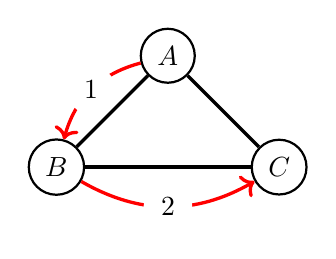
\begin{tikzpicture}[node distance= 2cm]
      \begin{scope}[every node/.style={circle,thick,draw}]
        \node (A) {$A$};
        \node (B) [below left of= A] {$B$};
        \node (C) [below right of=A] {$C$};
      \end{scope}
      \begin{scope}
        [every edge/.style={draw= black, very thick},
        every node/.style={fill= white,circle}]
        \path (A) edge (B);
        \path (A) edge (C);
        \path (B) edge (C);
        \path[->] (A) edge[draw= red, bend right= 30] node {$1$} (B);
        \path[->] (B) edge[draw= red, bend right= 30] node {$2$} (C);
      \end{scope}
    \end{tikzpicture}
  \end{center}
\end{eg}

\begin{defn}
  \label{defn:reachability}
  Let $G = (V,E)$ be a graph.
  For any two vertices $u,v \in V$, $u$ and $v$ are said to be \emph{s-t reachable} if there is a path from $u$ to $v$.
\end{defn}

\begin{eg}
  \label{eg:reachability-example-1}
  Consider the following (undirected) graph:
  \begin{center}
    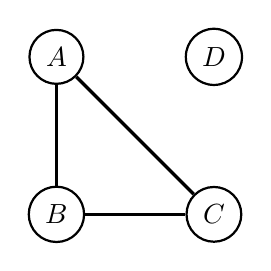
\begin{tikzpicture}[node distance= 2cm]
      \begin{scope}[every node/.style={circle,thick,draw}]
        \node (A) {$A$};
        \node (B) [below of= A] {$B$};
        \node (C) [right of= B] {$C$};
        \node (D) [right of= A] {$D$};
      \end{scope}
      \begin{scope}
        [every edge/.style={draw= black, very thick},
        every node/.style={fill= white,circle}]
        \path (A) edge (B);
        \path (A) edge (C);
        \path (B) edge (C);
      \end{scope}
    \end{tikzpicture}
  \end{center}
  $A$ and $C$ are s-t reachable.
  There are two paths connecting them (blue and red, respectively):
  \begin{center}
    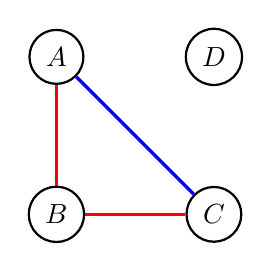
\begin{tikzpicture}[node distance= 2cm]
      \begin{scope}[every node/.style={circle,thick,draw}]
        \node (A) {$A$};
        \node (B) [below of= A] {$B$};
        \node (C) [right of= B] {$C$};
        \node (D) [right of= A] {$D$};
      \end{scope}
      \begin{scope}
        [every edge/.style={draw= black, very thick},
        every node/.style={fill= white,circle}]
        \path (A) edge[draw= red] (B);
        \path (A) edge[draw= blue] (C);
        \path (B) edge[draw= red] (C);
      \end{scope}
    \end{tikzpicture}
  \end{center}
\end{eg}

\begin{ceg}
  \label{ceg:reachability-nonexample-1}
  Consider the same graph defined in \cref{eg:reachability-example-1}, the vertices $A$ and $D$ are not s-t reachable.
\end{ceg}

\begin{thm}
  \label{thm:reachability-is-an-equivalence}
  Let $G = (V, E)$ be an undirected graph.
  The s-t reachability relation defined in \cref{defn:reachability} is an equivalence relation on the set of vertices $V$.
\end{thm}
\begin{proof}
  (Reflexivity): Let $v \in V$.
  The empty walk is trivially a path.
  Thus, $v$ is s-t reachable from itself.
  
  (Symmetry): Let $u,v \in V$ be any two vertices.
  Assume that $v$ is s-t reachable from $u$, i.e., there is a path $p$ from $u$ to $v$.
  We need to prove that $u$ is s-t reachable from $v$, i.e., there is a path from $v$ to $u$.
  To this end, we do induction on the length of $p$.
  In the base case, $p$ has length 0, so it is the empty path.
  Thus, the result follows from reflexivity.
  In the induction step, $p$ is a path of length $k+1$ and it is of the form $p',(u',v),v$, where $u'$ is some vertex and $p'$ is a path from $u$ to $u'$ of length $k$.
  By the induction hypothesis, there is a path $\widetilde{p}$ from $u'$ to $u$.
  Since $G$ is undirected, $(v,u')$ is also an edge of $G$.
  Thus, the sequence
  \[
    v,(v,u'),\widetilde{p}
  \]
  defines a path from $v$ to $u$.

  (Transitivity): Let $u,v,w \in V$ be any three vertices.
  Assume that there is a path $p$ from $u$ to $v$ and a path $p'$ from $v$ to $w$.
  The concatenation of $p$ and $p'$ defines a path from $u$ to $w$.
  You can prove this rigorously by induction on the length of $p$.
  The detail is left as an exercise.
\end{proof}

\begin{rmk}
  \label{rmk:reachability-not-equivalence-for-directed-graphs}
  In general, \cref{thm:reachability-is-an-equivalence} fails to hold for directed graphs because the s-t reachability relation is, in general, not symmetric.
\end{rmk}

\begin{ceg}
  \label{ceg:reachability-not-equivalence-for-directed-graphs-nonexample-1}
  Consider the following graph.
  \begin{center}
    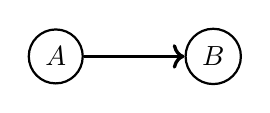
\begin{tikzpicture}[node distance= 2cm]
      \begin{scope}[every node/.style={circle,thick,draw}]
        \node (A) {$A$};
        \node (B) [right of= A] {$B$};
      \end{scope}
      \begin{scope}
        [every edge/.style={draw= black, very thick},
        every node/.style={fill= white,circle}]
        \path[->] (A) edge (B);
      \end{scope}
    \end{tikzpicture}
  \end{center}
  There is a path from $A$ to $B$, but there is no path from $B$ to $A$.
\end{ceg}

\begin{defn}
  \label{defn:connected-components}
  Let $G$ be an undirected graph.
  A \emph{(path) connected component} of $G$ is an equivalence class with respect to the s-t reachability relation.
\end{defn}

\begin{eg}
  \label{eg:connected-components-example-1}
  The graph defined in \cref{eg:reachability-example-1} has exactly 2 connected components (red and blue, respectively).
  \begin{center}
    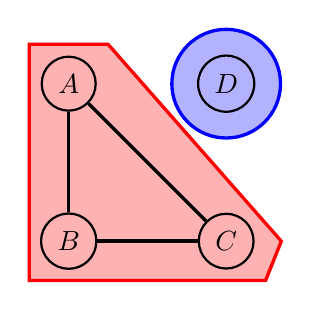
\begin{tikzpicture}[node distance= 2cm]
      \begin{scope}[every node/.style={circle,thick,draw}]
        \node (A) {$A$};
        \node (B) [below of= A] {$B$};
        \node (C) [right of= B] {$C$};
        \node (D) [right of= A] {$D$};
      \end{scope}
      \begin{scope}
        [every edge/.style={draw= black, very thick},
        every node/.style={fill= white,circle}]
        \path (A) edge (B);
        \path (A) edge (C);
        \path (B) edge (C);
      \end{scope}
      \begin{scope}[on background layer]
        \node[circle, draw=blue, very thick, fill= blue!30, fit= (D)] {};
      \end{scope}
      \begin{scope}[on background layer]
        \filldraw[red!30, draw=red, very thick] (-0.5,-2.5) -- (2.5,-2.5) -- (2.7,-2) -- (0.5,0.5) -- (-0.5,0.5) -- cycle;
      \end{scope}
    \end{tikzpicture}
  \end{center}
\end{eg}

\begin{defn}
  \label{defn:connected-graphs}
  An undirected graph $G$ is said to be \emph{(path) connected} if it has exactly one connected component.
\end{defn}

\begin{eg}
  \label{eg:connected-graphs-example-1}
  The graph defined in \cref{eg:graphs-example2} is connected because it has exactly one connected component.
\end{eg}

\begin{ceg}
  \label{ceg:connected-graphs-nonexample-1}
  The graph defined in \cref{eg:reachability-example-1} is not connected because it has two connected components.
\end{ceg}

\section{Graph exploration algorithms}
\label{sec:graph-exploration-algorithms}

\begin{rmk}
  \label{rmk:graph-exploration-algorithms-main-idea-1}
  To explore every vertex of an undirected graph $(V,E)$, we divide $V$ into two piles: frontier and unexplored.
\end{rmk}

\begin{rmk}
  \label{rmk:graph-exploration-algorithms-main-idea-2}
  If the unexplored pile is empty, then that means every vertex has been explored.
  We can remove everything from the frontier pile.
\end{rmk}

\begin{rmk}
  \label{rmk:graph-exploration-algorithms-main-idea-3}
  If the frontier pile is empty, move an arbitrary vertex in the unexplored pile to the frontier pile.
\end{rmk}

\begin{rmk}
  \label{rmk:graph-exploration-algorithms-main-idea-4}
  If the frontier pile is not empty, pick the next vertex $v$ in the frontier pile and move every vertex adjacent to $v$ in the unexplored pile to the frontier pile.
  At this point, $v$ has been fully explored, so we can remove $v$ from the frontier pile.
\end{rmk}

\begin{rmk}
  \label{rmk:graph-exploration-algorithms-next-vertex}
  The ``next vertex'' in \cref{rmk:graph-exploration-algorithms-main-idea-4} is intentionally abstract.
  There are two natural ways to pick the ``next vertex:'' pick the first vertex or the last vertex added to the frontier pile.
  The former choice corresponds to breadth-first search (BFS) and the latter choice corresponds to depth-first choice (DFS).
\end{rmk}

\begin{eg}
  \label{eg:bfs-example}
  Consider the following graph:
  \begin{center}
    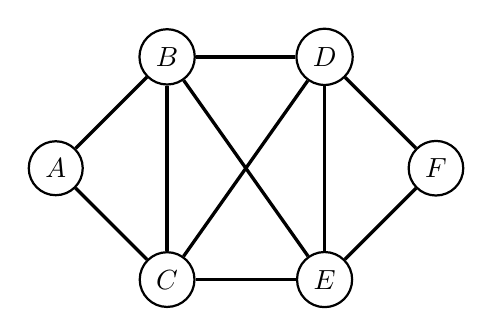
\begin{tikzpicture}[node distance= 2cm]
      \begin{scope}[every node/.style={circle,thick,draw}]
        \node (A) {$A$};
        \node (B) [above right of= A] {$B$};
        \node (C) [below right of= A] {$C$};
        \node (D) [right of= B] {$D$};
        \node (E) [right of= C] {$E$};
        \node (F) [below right of= D] {$F$};
      \end{scope}
      \begin{scope}
        [every edge/.style={draw= black, very thick},
        every node/.style={fill= white,circle}]
        \path (A) edge (B);
        \path (A) edge (C);
        \path (B) edge (C);
        \path (B) edge (D);
        \path (B) edge (E);
        \path (C) edge (D);
        \path (C) edge (E);
        \path (D) edge (E);
        \path (D) edge (F);
        \path (E) edge (F);
      \end{scope}
    \end{tikzpicture}
  \end{center}
  We run BFS on this graph.

  (Step 1): The frontier pile is empty and the unexplored pile consists of every vertex in the graph.
  By \cref{rmk:graph-exploration-algorithms-main-idea-3} we move an arbitrary vertex, e.g, $B$, to the frontier pile.
  \begin{center}
    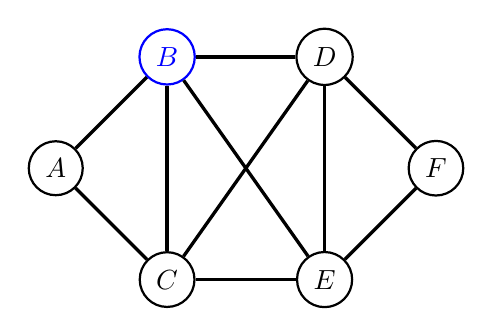
\begin{tikzpicture}[node distance= 2cm]
      \begin{scope}[every node/.style={circle,thick,draw}]
        \node (A) {$A$};
        \node[blue] (B) [above right of= A] {$B$};
        \node (C) [below right of= A] {$C$};
        \node (D) [right of= B] {$D$};
        \node (E) [right of= C] {$E$};
        \node (F) [below right of= D] {$F$};
      \end{scope}
      \begin{scope}
        [every edge/.style={draw= black, very thick},
        every node/.style={fill= white,circle}]
        \path (A) edge (B);
        \path (A) edge (C);
        \path (B) edge (C);
        \path (B) edge (D);
        \path (B) edge (E);
        \path (C) edge (D);
        \path (C) edge (E);
        \path (D) edge (E);
        \path (D) edge (F);
        \path (E) edge (F);
      \end{scope}
    \end{tikzpicture}
  \end{center}
  
  (Step 2): By \cref{rmk:graph-exploration-algorithms-main-idea-4}, pick the next vertex $B$.
  We have to move $A$, $C$, $D$, and $E$ to the frontier pile and remove $B$ from the frontier pile.
  \begin{center}
    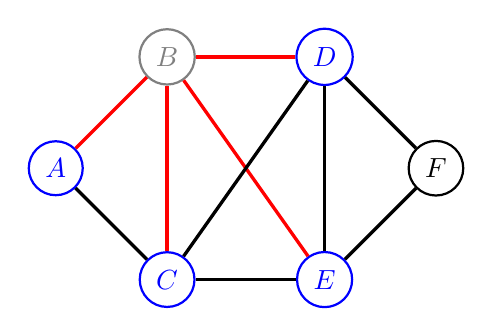
\begin{tikzpicture}[node distance= 2cm]
      \begin{scope}[every node/.style={circle,thick,draw}]
        \node[blue] (A) {$A$};
        \node[gray] (B) [above right of= A] {$B$};
        \node[blue] (C) [below right of= A] {$C$};
        \node[blue] (D) [right of= B] {$D$};
        \node[blue] (E) [right of= C] {$E$};
        \node (F) [below right of= D] {$F$};
      \end{scope}
      \begin{scope}
        [every edge/.style={draw= black, very thick},
        every node/.style={fill= white,circle}]
        \path (A) edge[red] (B);
        \path (A) edge (C);
        \path (B) edge[red] (C);
        \path (B) edge[red] (D);
        \path (B) edge[red] (E);
        \path (C) edge (D);
        \path (C) edge (E);
        \path (D) edge (E);
        \path (D) edge (F);
        \path (E) edge (F);
      \end{scope}
    \end{tikzpicture}
  \end{center}

  (Step 3): By \cref{rmk:graph-exploration-algorithms-main-idea-4}, pick the next vertex $A$.
  We do not have to move anything to the frontier pile because it is not adjacent to any unexplored vertex.
  Finally, we need to remove $A$ from the frontier pile.
  \begin{center}
    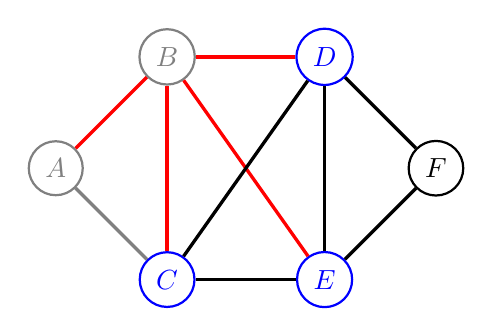
\begin{tikzpicture}[node distance= 2cm]
      \begin{scope}[every node/.style={circle,thick,draw}]
        \node[gray] (A) {$A$};
        \node[gray] (B) [above right of= A] {$B$};
        \node[blue] (C) [below right of= A] {$C$};
        \node[blue] (D) [right of= B] {$D$};
        \node[blue] (E) [right of= C] {$E$};
        \node (F) [below right of= D] {$F$};
      \end{scope}
      \begin{scope}
        [every edge/.style={draw= black, very thick},
        every node/.style={fill= white,circle}]
        \path (A) edge[red] (B);
        \path (A) edge[gray] (C);
        \path (B) edge[red] (C);
        \path (B) edge[red] (D);
        \path (B) edge[red] (E);
        \path (C) edge (D);
        \path (C) edge (E);
        \path (D) edge (E);
        \path (D) edge (F);
        \path (E) edge (F);
      \end{scope}
    \end{tikzpicture}
  \end{center}

  (Step 4): By \cref{rmk:graph-exploration-algorithms-main-idea-4}, pick the next vertex $C$.
  Again, we do not have to move anything to the frontier pile because it is not adjacent to any unexplored vertex.
  Finally, we need to remove $C$ from the frontier pile.
  \begin{center}
    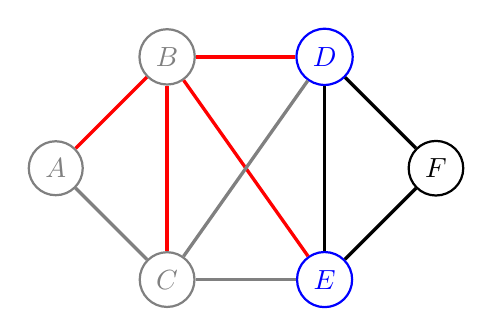
\begin{tikzpicture}[node distance= 2cm]
      \begin{scope}[every node/.style={circle,thick,draw}]
        \node[gray] (A) {$A$};
        \node[gray] (B) [above right of= A] {$B$};
        \node[gray] (C) [below right of= A] {$C$};
        \node[blue] (D) [right of= B] {$D$};
        \node[blue] (E) [right of= C] {$E$};
        \node (F) [below right of= D] {$F$};
      \end{scope}
      \begin{scope}
        [every edge/.style={draw= black, very thick},
        every node/.style={fill= white,circle}]
        \path (A) edge[red] (B);
        \path (A) edge[gray] (C);
        \path (B) edge[red] (C);
        \path (B) edge[red] (D);
        \path (B) edge[red] (E);
        \path (C) edge[gray] (D);
        \path (C) edge[gray] (E);
        \path (D) edge (E);
        \path (D) edge (F);
        \path (E) edge (F);
      \end{scope}
    \end{tikzpicture}
  \end{center}

  (Step 5): By \cref{rmk:graph-exploration-algorithms-main-idea-4}, pick the next vertex $D$.
  We need to move $F$ to the frontier pile and remove $D$ from the frontier pile.
  \begin{center}
    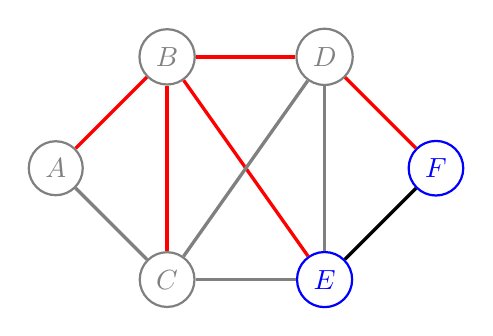
\begin{tikzpicture}[node distance= 2cm]
      \begin{scope}[every node/.style={circle,thick,draw}]
        \node[gray] (A) {$A$};
        \node[gray] (B) [above right of= A] {$B$};
        \node[gray] (C) [below right of= A] {$C$};
        \node[gray] (D) [right of= B] {$D$};
        \node[blue] (E) [right of= C] {$E$};
        \node[blue] (F) [below right of= D] {$F$};
      \end{scope}
      \begin{scope}
        [every edge/.style={draw= black, very thick},
        every node/.style={fill= white,circle}]
        \path (A) edge[red] (B);
        \path (A) edge[gray] (C);
        \path (B) edge[red] (C);
        \path (B) edge[red] (D);
        \path (B) edge[red] (E);
        \path (C) edge[gray] (D);
        \path (C) edge[gray] (E);
        \path (D) edge[gray] (E);
        \path (D) edge[red] (F);
        \path (E) edge (F);
      \end{scope}
    \end{tikzpicture}
  \end{center}

  (Step 6): The unexplored pile is empty.
  By \cref{rmk:graph-exploration-algorithms-main-idea-2}, we can remove everything from the frontier pile.
  \begin{center}
    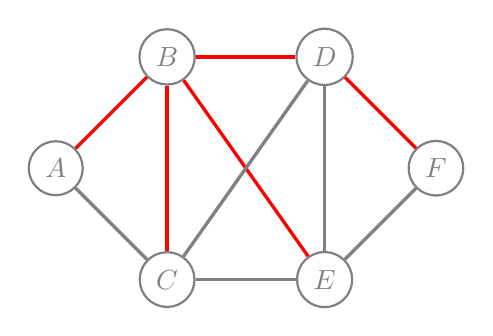
\begin{tikzpicture}[node distance= 2cm]
      \begin{scope}[every node/.style={circle,thick,draw}]
        \node[gray] (A) {$A$};
        \node[gray] (B) [above right of= A] {$B$};
        \node[gray] (C) [below right of= A] {$C$};
        \node[gray] (D) [right of= B] {$D$};
        \node[gray] (E) [right of= C] {$E$};
        \node[gray] (F) [below right of= D] {$F$};
      \end{scope}
      \begin{scope}
        [every edge/.style={draw= black, very thick},
        every node/.style={fill= white,circle}]
        \path (A) edge[red] (B);
        \path (A) edge[gray] (C);
        \path (B) edge[red] (C);
        \path (B) edge[red] (D);
        \path (B) edge[red] (E);
        \path (C) edge[gray] (D);
        \path (C) edge[gray] (E);
        \path (D) edge[gray] (E);
        \path (D) edge[red] (F);
        \path (E) edge[gray] (F);
      \end{scope}
    \end{tikzpicture}
  \end{center}
\end{eg}

\end{document}
